\documentclass[aspectratio=169]{beamer}
\usepackage{fontspec}
\usepackage{wrapfig}
\setmainfont{CMU Serif}
\newfontfamily{\cyrillicfont}{CMU Serif}
\setsansfont{CMU Sans Serif}
\newfontfamily{\cyrillicfontsf}{CMU Sans Serif}
\setmonofont{CMU Typewriter Text}
\newfontfamily{\cyrillicfonttt}{CMU Typewriter Text}

%%% Fonts and language setup.
\usepackage{polyglossia}
%% Math
\usepackage{amsmath, amsfonts, amssymb, amsthm, mathtools} % Advanced math tools.

\usetheme{Rochester}
\usecolortheme[style=light]{Nord}
\usefonttheme{Nord}
\setbeamertemplate{navigation symbols}{}%remove navigation symbols


\usepackage{minted}
\usemintedstyle{nord}

\title{Программная реализация
(на языке JavaScript)
алгоритмов генерации ФОС
по математике 2023}
\subtitle{Математический факультет 3 курс}
\author{Суматохина Александра }
\date{}


%%% Polyglossia setup after (nearly) everything as described in documentation.
\setdefaultlanguage{russian}
\setotherlanguage{english}

\begin{document}
\maketitle

\begin{frame}{Существующие проблемы}
    \begin{itemize}
        %TODO: Тут написан какой-то бред
        \item Дефицит заданий для подготовки
        \item Списывание ответов учениками
        \item При появлении новых заданий в экзамене, дефицит материалов увеличивается в разы.
        \item Некоторые задания решаются слишком быстро, а их составление вручную занимает несоразмерно много времени.
    \end{itemize}
\end{frame}

\begin{frame}{Проект «Час ЕГЭ»}
    «Час ЕГЭ» — компьютерный образовательный проект, разрабатываемый с 2013года при математическом факультете ВГУ в рамках «OpenSource кластера» и предназначенный для помощи учащимся старших классов подготовиться к тестовой части единого государственного экзамена.
\end{frame}

\begin{frame}{Примеры генерации задач №10}
    \vspace{-0.5cm}
    \begin{figure}[t]
        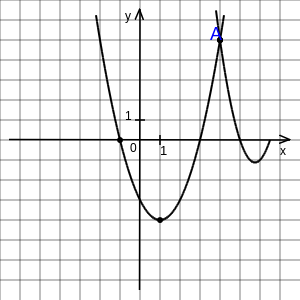
\includegraphics[scale=0.45]{images/449724462142151n0}
    \end{figure}
    На рисунке изображены графики функций $f(x)=2x^{2}-23x+65$ и $g(x)=ax^{2} +bx+c$, которые пересекаются в точках $A$ и $B$. Найдите ординату точки $B$.
    
\end{frame}

\begin{frame}{Примеры генерации задач №10}
    \vspace{-0.5cm}
    \begin{figure}[t]
    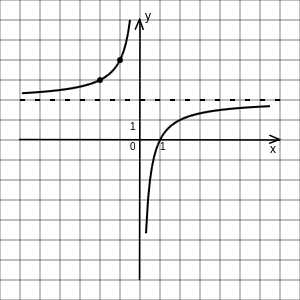
\includegraphics[scale=0.45]{images/610459930097164n0}
    \end{figure}
    На рисунке изображён график функции $f(x)=\frac{k}{x}+b$. Найдите $f(-20)$.
\end{frame}

\begin{frame}{Примеры генерации задач №10}
    \vspace{-0.5cm}
    \begin{figure}[t]
    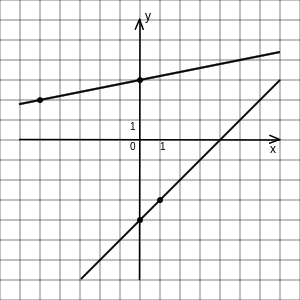
\includegraphics[scale=0.45]{images/1971545344438219n0}
    \end{figure}
    На рисунке изображёны графики двух линейных функций. Найдите ординату точки пересечения графиков.

\end{frame}

\begin{frame}{Этапы генерации}
    \begin{itemize}
        \item Генерация коэффициентов функций
        \item Подсчёт количества точек в узлах целочисленной решётки (функция \texttt{intPoints})
        \item Отрисовка целочисленной сетки и осей координат (функция drawCoordinatePlane)
        \item Отрисовка фунций с помощью функции (функция \texttt{graph9AdrawFunction})
    \end{itemize}
    
\end{frame}

\begin{frame}{Пример Ларина}

    \vspace{-0.5cm}
    \begin{figure}[t]
        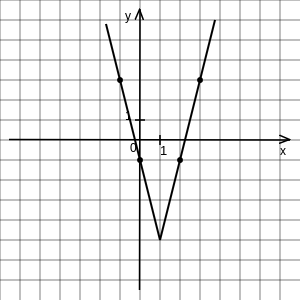
\includegraphics[scale=0.45]{images/453912618511153n0}
    \end{figure}
    На рисунке изображён график функции вида $f(x)=|kx+b|+c$, где числа $b$, $c$ и $k$ — целые, $k \leq 0$, $b\geq0$. Найдите сумму $k+b+c$.\vspace{2.5cm}

\end{frame}


\begin{frame}{Достижения}
    \begin{itemize}
        \item Полностью покрыт открытый банк заданий ФИПИ
    \end{itemize}
    
\end{frame}

\begin{frame}{Примеры генерации задач №7}
    \vspace{-0.5cm}
    \begin{figure}[t]
        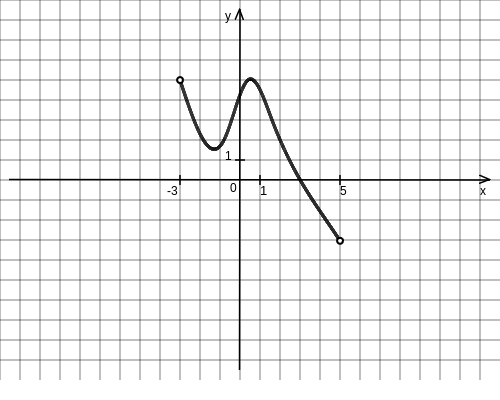
\includegraphics[scale=0.38]{images/9299084059373277n0}
    \end{figure}
    На рисунке изображён график $y=f'(x)$ — производной функции $f(x)$, определенной на интервале $(-3;5)$. В какой точке отрезка $[2; 3]$ функция $f(x)$ принимает наибольшее значение?
\end{frame}

\begin{frame}{Примеры генерации задач №7}
    \vspace{-0.5cm}
    \begin{figure}[t]
        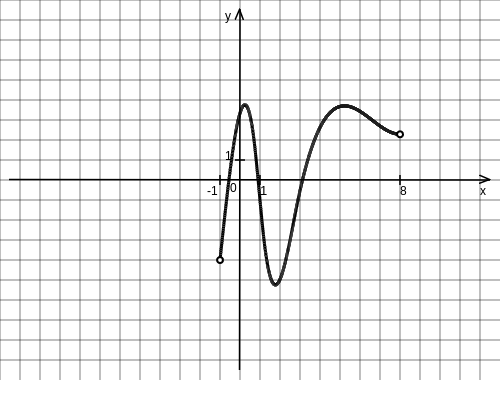
\includegraphics[scale=0.38]{images/776525944899729n0}
    \end{figure}
    На рисунке изображен график производной функции $f(x)$, определенной на интервале $(-1; 8)$. Найдите количество точек, в которых касательная к графику функции $f(x)$ параллельна прямой $y=-3x+ 14{,}8 $ или совпадает с ней.
\end{frame}

\begin{frame}{Примеры генерации задач №7}
    \vspace{-0.5cm}
    \begin{figure}[t]
        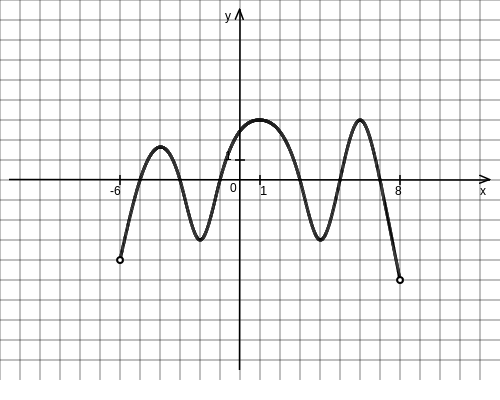
\includegraphics[scale=0.38]{images/020693809529216n0}
    \end{figure}
    На рисунке изображен график функции $y=f(x)$, определенной на интервале $(-6;8)$. Найдите сумму точек экстремума функции $f(x)$.
\end{frame}

\begin{frame}{Этапы генерации}
    \begin{itemize}
        \item Генерация точек, через которые будет проходить функция
        \item Использование сторонней библиотеки \texttt{Spline.js} для построение по точкам функции
        \item Проверка на нахождение графика в рамках видимости %что за бред?
        \item Нахождение количества экстремумов функции
        \item Отрисовка графика функции
    \end{itemize}
    
\end{frame}

\end{document}
